\chapter{Spatial Audio: Capture \& Reproduction}

\todo[inline]{I am not sure but I think this chapter is too long. I might need to split it into capture for one chapter and reproduction for another chapter. I can also just put reproduction into chapter 2. It might be ok.}

\section{Introduction}

This chapter will be developed with Tamara Smyth. In this chapter, we will shift the focus from spatial music to spatial audio. We will begin by drawing a line from the inception of recorded sound to the latest developments in 3D audio, including advancements in cross-talk cancellation (XTC), WFS, and ambisonics. In this chapter, we are concerned with the variety of ways that sound engineers can use spatial audio technologies to record and reproduce spatial music: whether that be in real-time or asynchronously. We will also touch upon some of the technical complications of this work that might prove problematic for engineers (ie. insufficient memory, speaker count, hardware requirements, etc.).

In particular, this chapter will focus on the main technology this author is concerned with: ambisonics. One of the major benefits of ambisonics is the \textit{isotropic}\footnote{Identical in all directions; invariant concerning direction. In an ambisonic context, this means the sound field can be reproduced in whatever sound system is available.} nature of the design, which makes it more flexible than surround sound standards such as 5.1. Ambisonics has a long-established tradition in the spatial audio community and as such, a myriad of open source tools have already been developed for its usage. These tools make it more accessible in many ways that \textit{object-based audio} (OBA) ecosystems. With the proliferation of systems for binaural rendering, ambisonics has resurfaced as a reliable method for spatial audio reproduction.

In addition to listing and demystifying the different spatial audio technologies available today for playback, we will suggest engineering approaches for the capture of spatial sound both for real-time transmission and for asynchronous dissemination using open-source technologies. We will focus on spatial audio recording techniques and describe systems based on freely available software for mixing and mastering spatial audio which can later be used in immersive environments such as the ones described in Chapter \ref{ch:xr-mus}. In contrast to Chapter \ref{ch:spat-mus}, which outlines technologies which are better suited for real-time performances with musicians, in this chapter we will focus more on tools for creating \textit{fixed-media} works.

\section{History of Spatial Audio Capture}

In the previous section of this paper we presented a number of composers who made space an integral part of their practice as well as \textit{spatial instruments} used for the development of such works. This next section will describe the development of modern spatial audio systems from an historical and engineering perspective. 

% Many engineers must be thanked for giving composers the ability to \textit{diffuse} sound in space towards musical ends. In this section we will discuss some of the most influential engineers that have contributed to the development modern \textit{spatial audio} systems. 

% The chapter will be divided into four sections: 

% \begin{enumerate}
%     \item Spatial audio developments before the 21st century
%     \item Contemporary spatial audio developments in sound recording
%     \item Contemporary spatial audio developments in sound reproduction
%     \item Overview of open tools for recording and playback of spatial sound
% \end{enumerate} 

\subsection{Audio Pioneers} \label{subsec:audio_pioneers}

The invention of the telephone, in 1876, by  Alexander Graham Bell \cite{grosvenor2016alexander}) can be considered the genesis of all \textit{spatial audio} technologies. The transmission principles it used where what later inspired the development of the phonograph, one of the first known recording devices, invented by Thomas Edison in 1877 \cite{gitelman1999scripts}, and, subsequently, galvanized a whole new generation of engineers who developed more sophisticated methods for sound capture and reproduction. 

\begin{figure}[ht]%force figure here, top, 
\centering
\includegraphics[width=0.7\textwidth]{img/theatrophone.jpeg} 
%\captionsetup{justification=centering}
\label{fig:theatrophone}
\caption{Théâtrophone \cite{theatrophone_pic}}
\end{figure}

A few years after the invention of recorded sound, Clement Ader, best known for his work in  aviation, would present the \textit{théâtrophone}, a "system of telephonic transmission where listeners received a separate channel for each ear, enabling stereophonic perception of actors on a set" during opera performances. Just a year before, Ader had presented his prototype at the Paris Exhibition for Electricity in 1881 \cite{malham19953}. Figure  \ref{fig:theatrophone} shows a picture of the device. We can see the two receivers which would be placed at the listeners ears for \textit{stereophonic} audition. The writing on the image also shows the cost for the audience member, which was 10 minutes for one franc, or 5 minutes, for 50 cents. 

Decades would pass before any new major developments in the field would occur, but eventually, in the 1920's, Harvey Fletcher, from Bell Telephone Laboratories\footnote{Bell labs has an important place in computer music history. It is where Max Mathews wrote the first computer music language, MUSIC-N.}, developed one of the first binaural recording systems. This system used the anatomy of the head to naturally embed spatial attributes of sound to recordings \cite{harvey1927binaural}. It would not be, however, until 1933, at the Chicago Century of Progress Exhibition, that binaural recordings would first be introduced to the public. 

Fletcher is believed to also be responsible for the first public demonstration of stereophonic sound, which took place in 1934 in New York City. Bell Telephone Laboratories, along with Fletcher, is also accredited for, in the 20's, being the first American institutions to research what is known today as wave-field synthesis (WFS): a system which captures a "wall of sound", using an array of microphones, and then consequently plays it back, using an array of speakers. In other words, engineers would mount a curtain of microphones and then reproduce the recorded signals using a curtain of speakers of similar proportions\cite{fletcher1942hearing}\footnote{While Fletcher would be one of the first to describe the idea of WFS in 1942, it would not be until 1988 that Berkhout would propose the mathematics involved in WFS to transform a single sound source into a wall of sound.}.

Later, in 1933, Fletcher also demonstrated the possibilities of long-distance multi-channel sound transmission. In a collaboration with English conductor Leopold Stokowski, considered one of the first stereo control-board operators\cite{mcginn1983stokowski}, Harvey and other Bell Lab engineers put together a system which transmitted the sound of an orchestra in Philadelphia via three microphones placed on stage to three corresponding loudspeakers in Washington DC's Constitution Hall. Bell Labs and Stokowski would go on to collaborate on numerous events in the 40's. Around the same time Alan Blumlein, an American engineer, was working on a much simpler yet powerful spatial audio technique: high-fidelity stereophony. 

Blumlein's most important contribution to the field of spatial audio is perhaps his mid-side (MS) encoding technique, patented in 1931 \cite{billingsley1987simulated}. This technique allowed audio engineers to mix stereo and mono information,  towards spread control, by summing and subtracting signals with equal and inverted phase. The technique was later expanded by Gerzon to develop a First Order Ambisonic\footnote{Also known as tetrahedral microphone} microphone. The idea consisted of taking the output of a \textit{figure-8} microphone and summing it with an \textit{omni-directional} microphone. A second copy of the figure-8 microphone would be phase inverted. The result were two cardioid like patterns with the same orientation as the stereo-speaker arrangement. Figure \ref{fig:ms_stereo} shows the general set-up for the MS stereo recording technique, note the panning on the two copies of the figure-8 microphone. 

\begin{figure}[h!]%force figure here, top, strict
\centering
\includegraphics[width=0.35\textwidth]{img/ms_stereo.svg.png} 
%\captionsetup{justification=centering}
\label{fig:ms_stereo}
\caption{Mid-Side Stereo \cite{ms_stereo_pic}}
\end{figure}

One of the biggest moments for spatial audio occurred at the very end of the decade. In 1940, Leopold Stokowski, RCA, and Disney would release the film \textit{Fantasia} which featured a system called \textit{Fantasound}. The control system they designed allowed audio tracks to be panned to any of 10 loudspeakers \cite{klapholz1991fantasia}. This lead to an era of development in professional theatre systems with much to be desired on the consumer end. Moderate improvements to sound quality and storage capacity were achieved from 1940 to 1970.

In the 1970's, a new and significantly more obscure technology began being developed: \textit{quadraphonic sound}. Quadraphonic research is believed to have begun at the Acoustic Research Corporation by Robert Berkovitz \cite{davis2003history}. The idea was to use two rear channels commercially to produce the ambience of the recording and two front channels for direct sound. Unfortunately, due to a number of financial, engineering, and marketing issues, the system never gained much popularity. Fortunately, the system did inspire other developments. 

The development of encoding and decoding schemes for quadraphonic sound would eventually peak the interest of British mathematician Michael Gerzon. Michael would, in 1969, present to the public a new audio capture method inspired by Alan Blumlein and the rise of interest in quadraphonics. Gerzon proposed, provocatively, the use of a tetrahedral array for audio capture in which the four signals could be encoded into three coincident\footnote{Coincident here meaning placed close together.} figure-8 microphones. This system, Gerzon believed, could optimize the use of the four speakers by providing listeners with not only horizontal information, but also vertical sound. Unfortunately, the system suffered from a considerably small ideal listening area\footnote{Also called \textit{sweet spot}. Higher Order Ambisonics (HOA) has been shown to increase the size of the sweet spot.}, a fact which detracted sound system engineers who were primarily concerned with audio for film, as it had become, and possibly remains, the focus of spatial audio research. 

Around the same time, in 1970, Tom Horall of what today is known as Acentech\footnote{https://www.acentech.com/} decided to attempt to recreate the acoustics of the famous Boston Symphony Hall using a acoustic model approximation. The system used tape delay techniques to achieve believable spatial sound. Using a dozen loudspeakers Horall was able to convince the listeners that they were actually being transported to the iconic hall. The system would later be commercialized in 1988 and become known as the Pioneer DSP-3000 \cite{davis2003history}. 

Many other developments followed suit from the 80's to today. Perhaps the most popular of these is 5.1 surround sound, a popular audio system which has had decent success commercially. Today, there is an ongoing battle regarding the future of spatial audio. Companies are consistently looking for scalable and reliable solutions to improve sound quality for patrons. Unfortunately, many of these systems have suffered from their distinctly complicated set-up process or high costs. The quest for: simple, high-fidelity, three-dimensional sound; is one that will, likely, not end soon. 

%\subsection{Stereo Techniques}
\subsection{Binaural Microphones}

\textit{Binaural audio} and \textit{multi-channel stereophony} are the two most common spatial audio technologies. \textit{Binaural audio} has become increasingly popular for \textit{virtual reality} (VR) while \textit{multi-channel stereophony} can be found in home entertainment systems as well as automotive sound systems. Stereo, however, is still the prevailing reproduction format, which is why binaural microphones have gotten some interest as a means of "static" spatial audio reproduction. Others have written about \textit{transaural} sound systems, which reproduce \textit{binaural audio} over stereo systems. \textit{Transaural} reproduction is a niche system that has been gaining more interest in the community. The underlying technology, however, seems to remain limited to audiophiles and a number of select engineers working on it.

In contrast to other spatial audio recording methods which rely on large arrays of microphones binaural recordings only use two microphones to encode spatial information into a stereo recording. Binaural recordings are either captured using a \textit{dummy-head}, a mannequin head with microphones inside its ears, or with \textit{in-ear} microphones placed inside a person's ear canals, to capture what they would normally listen to. By playing back these binaural recordings using headphones, ear-buds, or with stereo speakers using \textit{cross-talk cancellation} (XTC) filters\footnote{XTC is also referred to as \textit{transaural reproduction} in the literature.}, a person can sense a sonic space around them as it originally occurred. 

Unfortunately, some issues arise from this method. Firstly, people's heads and ears differ in size and shape, a fact which distorts the recordings ever so slightly breaking the illusion that one has been transported from their current location to the new auditory scene. Secondly, when the listener hears back the recording, they will be striped of rotational control. In other words, when they turn their heads, the sound will remain fixed in the same perspective as the original recording, and the illusion of immersion will be lost. This lack of \textit{auditory parallax} creates localization errors and \textit{internalization} of sound sources. Figure \ref{fig:dummy-head} shows a "dummy head" - a binaural microphone with two capsules placed inside the modeled pinnae, mimicking the behavior of the human cochlea\footnote{The biological structure in our inner ear where frequency analysis is performed.}. The \textit{pinnae} in these systems tends to be manufactured using a soft plastic such as silicone to mimic the absorption of human cartilage on sound.

\begin{figure}[ht!]%force figure here, top, strict
\centering
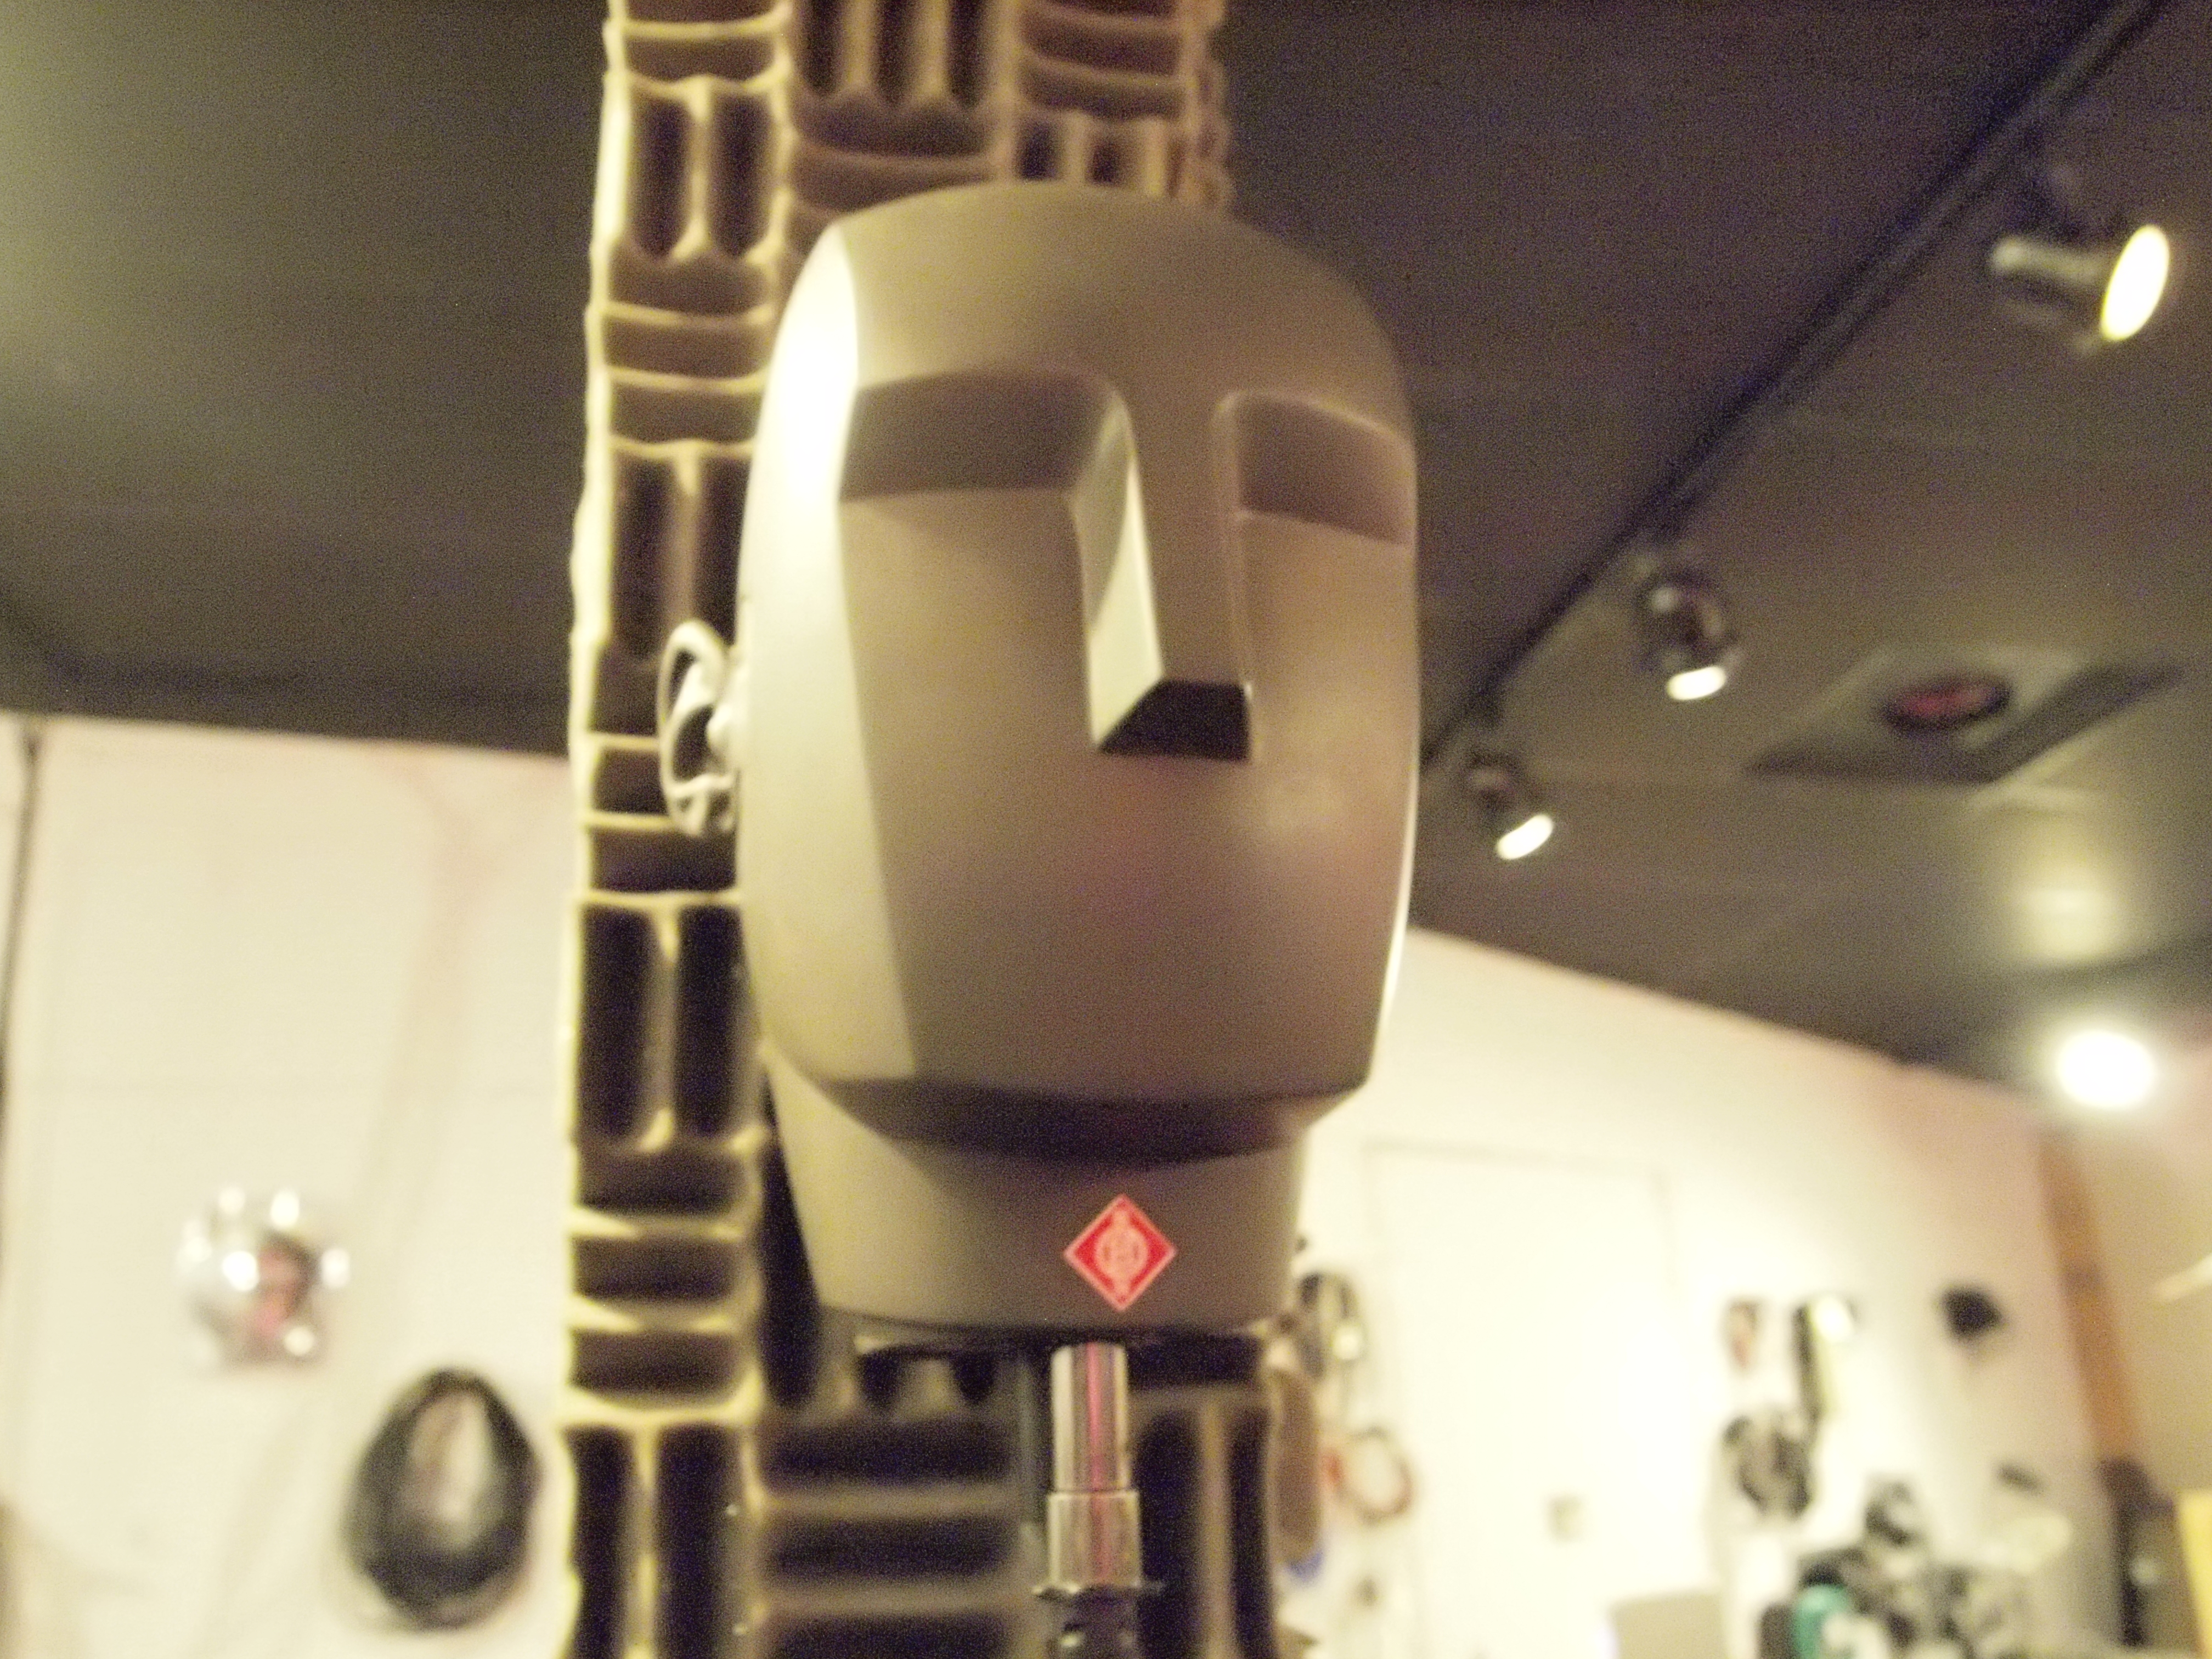
\includegraphics[width=0.7\textwidth]{img/dummy-head.jpg} 
%\captionsetup{justification=centering}
\label{fig:dummy-head}
\caption{Dummy Head - wikimedia commons}
\end{figure}

\textit{Binaural recordings} are not a particularly good representation of the desired soundfield resulting from a \textit{spatial music} work, however, they are crucial for the development of binaural synthesis systems, which ultimately can convey a proper representation of the musical work. Often, it becomes impractical to use a real human for HRTF sampling since the process can take quite a long time and human movements during acoustic sampling can lead to errors in the dataset. In this context, an anthropomorphic average of a human is better suited for the sampling task. Alternatively, the binaural impulse responses can be synthesized using acoustic models. \cite{algazi2002use}, for example, describes a head-and-torse model, or "snowman" model, to efficiently implement HRTF approximations towards real-time spatialization. 

\begin{equation} \label{eq:conv-hrir}
\begin{array}{l}
x_{L}(n)=\sum_{p=1}^{P} x_{p}(n) * h_{L, \theta_{p}, \phi_{p}}(n) \\
x_{R}(n)=\sum_{p=1}^{P} x_{p}(n) * h_{R, \theta_{p}, \phi_{p}}(n)
\end{array}
\end{equation}

\cite{hacihabiboglu2017perceptual} provides a simple equation for the \textit{auralization} of a virtual signal via convolution with two HRIRs. This is equivalent to the process of filtering the source $x_p$ with a filter whose frequency response would be identical to the Fast Fourier Transform (FFT) of $h_{R, \theta_{p}, \phi_{p}}$ and $h_{L, \theta_{p}, \phi_{p}}$ respectively. The topic of \textit{binaural synthesis} will be further discussed in later sections, as it is a primary topic of this work, which warrants extensive discussion.

\subsection{Soundfield microphones}

History of soundfield microphones.

\section{Contemporary Spatial Audio Capture Techniques} \label{sec:contemp_audio_capture}

While the popularity of spatial music has become evident in the electro-acoustic domain, little effort seems to have been devoted by composers for the accurate representation of their music in a recorded format. Often, composers opt to use stereo recordings of their work, due to the complexity of spatial audio recording technologies or their lack of availability. While in previous sections of this work we have focused on technologies which allow the creation of spatial music, in this section we will focus on hardware and software which allows one to document their works, with differing degrees spatial quality retained, for public dissemination outside of the concert hall. 

\subsection{Multi-channel Spaced Microphone Arrays}
%https://www.dpamicrophones.com/mic-university/immersive-sound-object-based-audio-and-microphones

Before we can begin to understand contemporary 3D audio capture techniques we should discuss some fundamental microphone principles. All spaced microphone arrays rely on systems which turn air pressure changes into electrical currents and subsequently binary information, which represent these pressure changes as sampled in time. Most well-known \textit{monophonic} microphone types fall within the family of cardioids. The general equation for the family of cardioids is:

\begin{equation}
    \rho(\theta) = \alpha + (1-\alpha)cos(\theta)
\end{equation}

This equation, from \cite{ortolani2015introduction}, provides a way for us to construct the most common types of \textit{polar patterns} found in commercial microphones today. \textit{Polar patterns} depict the sensitivity of a microphone to sound pressure as a function of the direction-of-arrival (DOA) and are frequency dependent. The most important patterns for our purposes are: \textit{omni-directional} where $\alpha=1$ \textit{cardioid} where $\alpha = 0.5$, and \textit{figure-of-eight} where $\alpha=0$. Figures \ref{fig:card}, \ref{fig:omni}, and \ref{fig:fig-8} show the polar patterns of these three popular types of microphones. 

\begin{figure}[!htb]
\minipage{0.32\textwidth}
  \includegraphics[width=\linewidth]{img/card.png}
  \caption{Cardioid Polar Pattern \cite{card_pic}}\label{fig:card}
\endminipage\hfill
\minipage{0.32\textwidth}
  \includegraphics[width=\linewidth]{img/fig-8.png}
  \caption{Figure-8 Polar Pattern \cite{fig8_pic}}\label{fig:fig-8}
\endminipage\hfill
\minipage{0.32\textwidth}%
  \includegraphics[width=\linewidth]{img/omni.png}
  \caption{Omni Polar Pattern \cite{omni_pic}}\label{fig:omni}
\endminipage
\end{figure}

These idealized responses show the sensitivity of different microphones to sound waves arriving from different directions. For the cardioid\footnote{Which gets it's name from it's heart-shaped response.} pattern, we see a \textit{null} at 180\textdegree and \textit{unity} response at 0\textdegree. These diagrams are seldom true in real-life, especially for high frequencies. Even for very good omni-directional microphones, eventually the capsule size becomes comparable to that of the wavelength, making the response directional. 

\textit{Off-axis coloration} refers to microphone's difference in frequency response at different directions. Most microphones can intuitively be separated into \textit{side address} or \textit{front address} microphones based on their construction. For \textit{front address} microphones, the reported frequency response will likely be based on a measurement with the capsule facing the excitation source so the response matches the ergonomic use of the microphone. Any \textit{side address} microphone, such as a cardioid condenser microphone, would perform poorly if the musician oriented the microphone backwards, resulting in a different frequency response than expected.

\textit{Proximity effect} is another term which relates to the nature of unidirectional microphones\footnote{Cardioids and figure-8 microphones fall under this category.} to exhibit a bass-boost when placed too close to the source. This is why many condenser microphones come equipped with a bass roll-off switch. The bass-boost comes from the \textit{pressure gradient} microphone. At low enough frequencies, the wavelength is vastly larger than the microphone capsule, so the difference in pressure at either side can be unnaturally large. This effect should be considered when placing musicians in relation to the microphones.

The mid-side (MS) technique previously discussed is just one of several stereo techniques that are traditionally implemented for stereo recording. While other stereo techniques such as A/B, X/Y, and ORTF also exist, these fall outside the scope of this text. The reader is referred to \cite{lipshitz1986stereo} for a lively discussion on the merits of coincident and spaced arrays for stereo reproduction. It warrants mentioning that by no means are surround-sound techniques objectively superior. In fact, there is still a lot of research being undertaken in this domain, in particular by The University of Huddersfield \cite{lee3d}. 

\textit{Spaced arrays} are a family of microphone arrays designed originally for surround sound formats. Various authors over the years have experimented and documented their configurations in order to facilitate the creation of high-quality multi-channel music for film. Figure \ref{fig:c-spaced-arrays} shows five complete spaced arrays adapted from \cite{hacihabiboglu2017perceptual} and \cite{politis2016microphone}. The diagram created is a rough approximation of these five 5.1 arrays. In addition to these five arrays, ambisonic arrays are also considered complete \textit{coincident} arrays capable of encoding surround sound formats. \cite{Immersiv9:online} also provides information about these arrays\footnote{Distances and angles might be slightly different from one reference to another. \textbf{TODO}}.

% 5.1 arrays (Fukada Tree, INA-5, Hamasaki Tree, DPA 5100, OCT-surround)
\begin{figure}[ht!]%force figure here, top, strict
\centering
\includegraphics[width=1.0\textwidth]{img/complete-spaced-arrays.jpeg} 
%\captionsetup{justification=centering}
\label{fig:c-spaced-arrays}
\caption{Complete Spaced Arrays}
\end{figure}

\todo[inline]{The symbols I used for these drawings are not standard. Not sure if that is ok.}

In addition to the five depicted arrays:
\begin{enumerate}
    \item \textbf{Fukada Tree}
    \item \textbf{INA-5} 
    \item \textbf{Hamasaki Tree}
    \item \textbf{DPA 5100}
    \item \textbf{OCT-surround}
\end{enumerate}

% Front arrays (Optimal Cardioid Triangle, Decca Tree, INA-3). Rear arrays (Hamasaki Square, IRT Cross)

A secondary technique exists for multi-channel audio recordings which involves a combination of a proximal front array and a distant rear array. In this configuration it is up to the sound engineer to decide how distantly the rear array will be placed. The decision will be based generally on the size of the space as well as how diffuse the sound is at the set distance. Front arrays include: Optimal Cardioid Triangle, Decca Tree, and INA-3. Rear arrays include: Hamasaki Square, and IRT Cross. Figure \ref{fig:fnr-arrays} shows a coarse approximation the associated arrays.

\begin{figure}[ht!]%force figure here, top, strict
\centering
\includegraphics[width=1.0\textwidth]{img/front-n-rear-arrays.pdf} 
%\captionsetup{justification=centering}
\label{fig:fnr-arrays}
\caption{Front and Rear Arrays}
\end{figure}

\subsection{Encoding Monophonic Sources}

% The recording array from the grid mics are numbers 15+17, 18+20, and 27+30. Those mics are mixed in with the hanging ORTF pair, which moves from time to time. So that’s 6 available right now. 

The same principle of ambisonic panning, formerly introduced as a technique for creating spatial representations in music, can be extended as a recording technique for 3D audio scene construction. In this approach, rather than specifying the positions of the desired sound source trajectories, we define for the encoder the positions of the statically placed microphones used for the recording. For example, within our experimental concert hall at CPMC, it is possible to define a template with the location of our fixed microphone locations, used routinely for concert recording. By placing the appropriate channels in the location tracks with the corresponding panners, we can render the recordings in a multi-channel format for playback over headphones or multi-channel speaker systems. Figure \ref{fig:cpmc122-mic-grid} shows the positions of 6 microphones typically used by our house engineers for multi-track recording. An additional ORTF pair located at the center of the grid is also included in the multi-track recordings, however, the position of this pair is not perpetually fixed\footnote{According to our house engineer.}. 

\begin{figure}[h!]%force figure here, top, strict
\centering
\includegraphics[width=0.5\textwidth]{img/cpmc122-mics.jpg} 
%\captionsetup{justification=centering}
\label{fig:cpmc122-mic-grid}
\caption{CPMC122 Microphone Grid - UCSD Dept. Music}
\end{figure}

A common technique implemented by recording engineers is combining multi-channel microphone arrays with fixed microphones. In the aforementioned case the 6 microphones are distant from our musicians and as a result they pick up sounds from all instruments on stage. In order to isolate sources, giving us more control in post-production, \textit{spot microphones} can be placed closer to the musicians. Ideally, the distances of all these fixed receivers are calculated in relation to the ideal listening position, both in terms of azimuth and elevation. 

\subsection{Coincident Microphone Arrays}

Of primary importance to our work is the development and optimization of coincident microphone arrays. Coincident microphone arrays come in various shape and sizes. The predominant characteristic of these devices is that proximity between sensors is minimized in order to improve localization estimations and the operating frequency \textit{virtual microphones} created by combinations of signals. There are three main types of coincident microphone arrays we were able to discern from the literature: spherical microphone arrays, studio microphone arrays, and planar microphone arrays. While most planar microphone arrays are not meant for high-quality studio recordings, we will nonetheless cover them here since many use similar operational conditions as the proposed HOA system being developed by the author. 
\subsubsection{Planar Microphone Arrays}

Planar microphone arrays are a subset of coincident microphone arrays which attempt to sample a soundfield using either a linear (one-dimensional arrays), or circular array (two-dimensional arrays). Most planar microphone arrays, although not all, fall under tha category of arrays for \textit{noise suppression}, as opposed to studio arrays for multi-channel recording. These devices tend to output a single audio channel that is the sum of various sensors delayed based on the desired direction of sound capture. 

\cite{backman2006miniature} provides some insight into planar microphone arrays and their relationship to soundfield microphones. The author in that publication relies on Micro-Electrical Mechanical Systems (MEMS) capsules for his designs. Backman suggests using multiple transducers to improve signal-to-noise ratio (SNR) and improve polar pattern control over the entire audio bandwidth (20Hz-20kHz). In a second paper \cite{backman2006gradient} the author expanded upon the theoretical work proposing a 5.1 planar array based on MEMS. Unfortunately, little information was presented regarding a 3D audio capture system - the designs described were predominantly for 2D audio. 

\todo[inline]{I want to come back to these Backman papers and add more detail. There are some useful equations there. Unless they are covered more clearly in other papers.}

\cite{chen2015theory} provides a more thorough review of planar arrays. Chen's paper describes a 2D planar array designed with first order microphones which can suitably sample vertical elements of the soundfield. The benefit of planar arrays is that for certain applications, spherical arrays simply might not be possible to construct, such as in cellphone or tablet designs. One noteworthy process implemented in this publication, as well as several others, is the use of simulated responses to validate designs prior to implementation. The main problem we found with this design was the limited bandwidth which had a maximum frequency of 850Hz. For high-quality audio purposes, we seek instead to operate on the audible frequency range. Secondly, in order to sample vertical harmonics, the number of transducers had to be increased from nine, the minimum number required for 2OA\footnote{Second order ambisonics.}, to 16, which increases the cost of the final design. 



% As the author suggests, most authors today are less interested in horizontal only audio capture, and even less so in systems which only sample the soundfield in 1D - likely because surround sound has encouraged the creation of material with 2D qualities. Extending WFS to a 2D representation yields a similar representation to that generated by VBAP \cite{smith2019spatial}. 

% Planar microphone arrays have nonetheless become increasingly popular as systems for direction-of-arrival (DOA) estimation and subsequent beamforming operations. In these systems, the linear microphone array is used to estimate the DOA of a signal using statistical analysis of the signals. Then, a beamforing operation can be performed on these same signals to generate a highly directive microphone pattern \textit{pointing} at specified location. This can be used, for example, to isolate and improve the quality of recording for a speaking person within a noisy environment. The same principle has also been applied to circular and spherical arrays. 

\subsubsection{Spherical Microphone Arrays}

Spherical microphone arrays are particularly interesting to us because they represent a simple way of capturing spatial sound both in a studio setting and in nature. In contrast to other recording techniques in which musician coordinates need to be defined in order to create a adequate soundfield, spherical microphone arrays inherently encode this information into what are called A-format recordings which are then encoded into the spherical domain for reproduction over an arbitrary loudspeaker or binaural system. 

Spherical microphone arrays can further be separated into three types of arrays: rigid, hollow, and tiered. Tiered arrays constitute arrays in which various radii are superimposed in order to capture different regions of interest of the soundfield (cite). In general, these systems have gotten less attention due to the difficulty of integrating these models with camera systems. Rigid and hollow models are more popular, and corresponding mathematical formulations exist for both. At their names suggest, a rigid spherical microphone array has no cavities exposed to the outside of the array, while the hollow designs do have open spaces over which sound may propagate.

In general, it rigid microphone arrays have gotten the most attention from the commercial sector, because of the elegance of their complimentary design with multi-camera systems, however, hollow arrays have also been implemented commercially in audio-only designs, targeted towards audio engineers who are not interested in producing video content. 

\subsubsection{Studio Microphone Arrays}
%This section describes some studio coincident microphone arrays. 
These are all studio techniques in which microphones are placed as close together as physically possible. 

Native B-format array, double MS, double MSZ, etc.

\subsection{Arrays in series}
A modern type of sound capture technique has recently been developed and is the subject of great interest for spatial audio researchers. The technique, predominantly employed under the basis of ambisonic rendering, involves capturing multiple soundfields simulateneously using an \textit{array of arrays}. In other words, a recording engineer positions a grid of multiple spaced microphone arrays in such a way that the \textit{acoustic boundaries} of adjacent arrays overlap each other. 

The goal of this capture technique is to allow, within a digital representation, six degrees of freedom (6DoF), or, \textit{translational} movement, in addition to the standard rotational control. Figure \ref{fig:6DoF} shows these translational transformations where yaw, pitch, and roll correspond to rotational transformations. 

\begin{figure}[h!]%force figure here, top, strict
\centering
\includegraphics[width=0.5\textwidth]{img/6DOF.svg.png} 
%\captionsetup{justification=centering}
\label{fig:6DoF}
\caption{6DoF - wikimedia commons}
\end{figure}

\section{Open Tools for Spatial Audio Capture}

A number of authors have described the development of Free and Open Source Hardware (FOSH) for the capture of real soundfields for either asynchronous or synchronous transmission. The majority of these designs fall under the category of spherical microphone arrays although other projects exist which discuss alternative geometries for spatial audio capture. While many publications have been presented wherein the authors describe the creation of such systems, few have actually sought to provide full documentation detailing the process undertaken to realize the entire system. 

A common problem with these designs for musicians seeking to enter the world of soundfield recording is the costly price-point of some of the Bills of Materials (BoMs) suggested by the engineers. In order to swap parts, the musician would need to know about electronics specifications and how to modify Computer Assisted Design (CAD) files in order to create his or her own systems.

\section{History of spatial audio reproduction}

\subsection{Stereophony}
seminal research into stereo reproduction
xtc (aka transaural)

\subsection{Quadraphony}
history of quad audio

\subsection{Surround Sound}
ITU standards, THX, MPEG-H, etc.

\section{Contemporary Spatial Audio Reproduction Techniques} \label{sec:contemp_audio_reproduction}

In the previous section we talked extensively about the artists and engineers who have shaped the way we think and talk about spatial sound. The various sections to follow will provide a look into some of the state-of-the-art research regarding spatial audio solutions and the: composers, institutions and practices, which are pushing us to further our understanding and curiosity. 

\subsection{Amplitude Panners}
\label{subsec:amplitude panner}

\todo[inline]{VBAP, DBAP, other panners, octo, quad, etc.}

Out of the various iterations of vector based systems the most prominent and well-regarded is called Vector Based Amplitude Panning (VBAP). In his 2001 paper (citation) Pulkii describes how trigonometric operations can be used to position a sound in any position in 3D space. The idea behind VBAP is to create \textit{phantom images} between sources giving listeners the illusion that sounds emanate from any arbitrary position between 2 or more speakers. Pulkii, the inventor of VBAP, from Helsinki, Finland, writes in regards to the difference between this method and ambisonic panning\footnote{Ambisonic panning does not use spherical microphones but encodes arbitrary audio sources for ambisonic reproduction.}: "the gain factor calculation in the VBAP method equals that of the Ambisonics in an orthogonal\footnote{Regular loudspeaker layouts.} loudspeaker placement". The key difference is that VBAP generalizes the calculation for all situations making it extremely flexible. While these two systems might seem remarkably similar, experiments have suggested that there exist statistically significant perceptual differences for both reproduction methods (Marentakis 2014). VBAP has gained much popularity among composers due to it's simplicity and elegance. A MAX/MSP collection of externals were developed by Pulkii in 2000 to allow electronic musicians to experiment with the system making it fairly accessible. It should be noted that as with many other spatialization methods it relies heavily on a great number of speakers for successful immersion. 

\subsection{Object Based Audio}
\label{subsec:oba}

Object based audio (OBA), or systems like it, are what most large spatial audio companies are invested and developing today. In many ways OBA, VBAP and ambisonic panning are similar in their approach yet differ slightly in their architecture and implementation. In OBA, an audio object contains metadata pertaining to it's position, time, and acoustic features. The metadata is used in soundtrack scoring for film and games and dictates the spatial attributes of the sound over time. While VBAP and Ambisonic encoded sounds can be panned in real-time, as OBA does, neither contain this information beforehand. OBA is used extensively in game engine development and is the leading format used by movie studios to develop sound for film. 

\subsection{Wave Field Synthesis}
\label{subsec:wfs}

Whilst less commonly seen or talked about, wave field synthesis (WFS) is another area of interest for acousticians and composers. WFS attempts to capture a wavefront and reproduce it at a later stage. A good case scenario for this is the simulation of a live concert. A wall of microphones is placed ten meters from the band and, at a later point, a wall of speakers is used to play back the recorded audio. A new audience could in theory listen to this reproduction and be transported to the event. The audience members could even walk around the "dance floor" and experience the rich spatial detail as if they were really there. WFS is a powerful spatial technique but entirely context dependent. It is often not desirable for situations in which sound arriving from all directions need to be captured. WFS also costly, as proper capture and reproduction takes dozens of microphones and speakers, making it inaccessible for most consumers.

\subsection{Higher Order Ambisonics}
\label{subsec:ambi}

Ambisonics is a full-sphere capture and reproduction method popular among spatial audio enthusiasts. A resurgence in interest, as with any of the aforementioned methods, can be attributed to the growth of mixed reality\footnote{MR: augmented reality in which digital objects can be interacted with}, augmented reality (AR) and virtual reality (VR) systems. Ambisonic has become of the de facto spatial audio reproduction methods in simple VR experiences, especially 360 video. 

Ambisonic signals can be created by panning traditional monophonic recordings or by capturing them via an ambisonic microphone. A tetrahedral microphone, the simplest ambisonic microphone, captures First Order Ambisonic (FOA) A-format\footnote{A-format audio is ambisonic audio prior to encoding.} signals which can be used to reproduce 360 degrees of spatial audio with tolerable quality. 

The theory and application of ambisonic heavily relies of the assumption that the playback system is composed of a spherical array of speakers which situates the listener at the origin. The tetrahedron shape is the lowest geometric approximation of a sphere, its shape is thus chosen for first order ambisonic capture. Higher approximations result in a higher number of channels and better spatial quality at the cost of more data to be handled and stored. The assembly and calibration of Higher Order Ambisonic (HOA) microphones remains a laborious and often HOA panning is used instead.

One of the major limitations of ambisonics recordings captured with these microphones, over other techniques - such as OBA - is the fact that the listener is confined to the geometric position in which the recording was taken in or synthesized for. In VR, AR and MR, users generally are not satisfied with being stationary - even if they can turn and tilt their head. These recordings work suitably well for viewers experiencing 360 videos, but if users want to traverse a digital playground, they will not be able to do so convincingly. It could therefore be said that whilst ambisonic can provide a good ambience layer for these experiences, it relies heavily on other strategies for full immersive experiences. Recent research efforts have focused on the interpolation \textit{between} soundfields, such that users can move around freely between various ambisonic recordings taken in proximity to each other. 

\subsubsection{Mathematical Formulation}

\subsubsection{Decoding Strategies}

\todo[inline]{beam forming}

\subsection{Binaural Synthesis}
\label{subsec:bin-synth}

% \subsection{Spherical Speaker Arrays}


\section{Open Tools for Spatial Audio Reproduction}

\todo[inline]{DAWs and VSTs, not CPU mus languages}

\cite{nettingsmeier2008ambi} provides us with a good description of the processes required to adequately set up an ambisonic playback system at home. We are interested in these particular solution not just because of the robustness of the method, but also because it was designed using all open source software. The benefit of open source software is that it is generally free, and, as a result, it lowers the overall cost of having to mount systems such as the one described. Naturally, a system like this one would still remain far more prohibitive than ambisonics over binaural synthesis within a WebVR experience - for example - but the comparison is really like comparing apples to oranges, WebVR, or any other commercial VR solution, is far from being able to achieve complete multi-modal\footnote{By multi-modal we mean: stimulating more than one sense. "Ideally" the experience would trick all five senses.} immersion.

In the aforementioned publication the author employs a hexagonal horizontal-only speaker set-up, however, it should be noted, the biggest benefit of ambisonics in the context of creating spatial music is the proliferation of binaural decoders for the method which allow one to forego speaker systems entirely\footnote{The quality of the final mix will be dependent on the quality of the binaural decoder.}. What this means is that if a composer is interested in creating music for HDLAs, they need not have access to a sophisticated loudspeaker system - they only need a pair of headphones and computer. In certain contexts, however, it is useful to have multi-channel systems operational and calibrated (for a spatial music class, for example). 

In such a case, where a "real" loudspeaker set-up is required Nettingsmeier, provides us with a good description of the associated steps required to calibrate such a system. Summarily, the steps in that paper are:

\begin{enumerate}
    \item Get all the gear you need, checking that: drivers for interfaces are supported by OS\footnote{You will need a decent amount of RAM. The higher order ambisonics the more RAM will be needed.}.
    \item Organize the number of speakers you have available in the desired layout (in his case a hexagon). 
    \item Measure the distances and angles from the center position and adjust speakers so the vertices of the ideal polygon (or polyhedron) match the mathematical model.  
    \item With the measured angles and distances, create a decoder using the AmbDec by Fons Adriansen\footnote{For Linux only. See ambi-X, IEM Plug-in Suite, or ATK for other systems.}.
    \item Use Aliki and Digital Room Correction (DRC) software to create six correction filters\footnote{This requires a good quality omni mic, such as the umik-1 by miniDSP (used in our work). Alternatively one can borrow a Earthworks M30, or similar measurement microphone from their University.}.
    \item Use an RMS meter to "level match" all your speakers. For this step and the last the center of the "rig" should be the reference point. 
    \item Listen and modify based on your preference. You can change your mind and build a new decoder, or remove speakers if you want. 
\end{enumerate}

\begin{figure}[ht]%force figure here, loosely
\centering
\includegraphics[width=1.0\textwidth]{img/nettingsmeier-extra-frontal.png} 
%\captionsetup{justification=centering}
\caption{Nettingsmeier Ambi System}
\label{fig:extra-frontal}
\end{figure}

Figure \ref{fig:extra-frontal} shows the signal flow for Nettingsmeier's simple home ambisonic system. We chose to generalize the signal flow since the choice of hardware is mostly irrelevant, and we seek to understand a framework that is modular and flexible. The correction filters mentioned are created to counter the imperfect frequency reproduction of the speakers as well as the effects of room acoustics. The \href{https://jackaudio.org/}{Jack software} is used to connect different associated audio algorithms for the final reproduction. It should be noted that this solution was presented over ten years ago, since then other software packages have been released which allow for more streamlined FOS\footnote{Free and open source.} ambisonics. 


\section{Conclusion}